\documentclass[a4paper,10pt]{article}

% Paquetes y configuración básica
\usepackage[utf8]{inputenc}
\usepackage[T1]{fontenc}
\usepackage{lmodern}
\usepackage[spanish]{babel}
\usepackage{amsmath,amssymb}
\usepackage{graphicx}
\usepackage{float}
\usepackage{caption}
\usepackage{listings}
\usepackage{color}
\usepackage{hyperref}
\usepackage{geometry}
\usepackage{fancyhdr}

% Configuración de márgenes
\geometry{left=3cm, right=3cm, top=2cm, bottom=2cm}

% Encabezado y pie de página (adaptado a la plantilla de referencia)
\pagestyle{fancy}
\fancyhead[L]{Template for Nonlinear Analysis, Modelling and Control}
\fancyhead[R]{\today}
\fancyfoot[C]{\thepage}

% Configuración de listings para código Python
\definecolor{codegray}{rgb}{0.5,0.5,0.5}
\definecolor{codepurple}{rgb}{0.58,0,0.82}
\definecolor{backcolour}{rgb}{0.95,0.95,0.92}
\lstdefinestyle{mystyle}{
    backgroundcolor=\color{backcolour},
    commentstyle=\color{codegray},
    keywordstyle=\color{blue},
    numberstyle=\tiny\color{codegray},
    stringstyle=\color{codepurple},
    basicstyle=\footnotesize\ttfamily,
    breaklines=true,
    captionpos=b,
    numbers=left,
    numbersep=5pt,
    showspaces=false,
    showstringspaces=false,
    showtabs=false,
    tabsize=4
}
\lstset{style=mystyle, language=Python}

% Datos del documento
\title{Reporte de Simulación en Python: Desplazamiento de Puntos y Cambio de Fondo}
\author{Alan Miranda, Cristian Orozco, Marlon Caviedes \\ \small{Infotep}}
\date{\today}

\begin{document}

\maketitle

\begin{abstract}
Este reporte muestra una simulación sencilla en Python en la que se desplazan puntos hacia la derecha. Si los puntos salen del área definida, se generan nuevos de forma aleatoria dentro del cuadro. Además, se cambia el color de fondo en cada paso de la animación. Aquí se explica el código, se muestran algunas imágenes de la simulación y se analizan brevemente los resultados.
\end{abstract}

\section{Introducción}
En este trabajo se exploró el uso de Python y Jupyter para crear animaciones simples con \texttt{matplotlib}. Se desarrolló una simulación donde unos puntos se mueven hacia la derecha en una gráfica. Cuando un punto se sale del límite del área, se genera de nuevo en una posición aleatoria. También se implementa un cambio en el color del fondo para hacer la animación más dinámica.

\section{Objetivos}
Los objetivos de esta actividad fueron:
\begin{itemize}
    \item Aprender a mover puntos de forma vectorizada en Python.
    \item Regenerar puntos que se salen del área.
    \item Cambiar el color del fondo durante la animación.
    \item Documentar el proceso en un reporte.
\end{itemize}

\section{Descripción de la Actividad y Código}
La simulación se basa en una clase llamada \texttt{Escena} que:
\begin{enumerate}
    \item Inicializa la escena con un tamaño específico, color de fondo y una cantidad de puntos generados aleatoriamente.
    \item Dibuja la escena de manera estática.
    \item Crea una animación en la que los puntos se desplazan hacia la derecha. Si algún punto se sale del límite, se le asigna una nueva posición aleatoria.
\end{enumerate}

El siguiente fragmento muestra el código principal:

\begin{lstlisting}[caption={Código en Python para la simulación}, label=lst:codigo]
import numpy as np
import matplotlib.pyplot as plt
import matplotlib.patches as patches
from matplotlib import animation

class Escena:
    def __init__(self, width, height, color, n_points):
        self.width = width
        self.height = height
        self.color = color
        self.n_points = n_points
        self.points = np.column_stack((
            np.random.uniform(0, width, n_points),
            np.random.uniform(0, height, n_points)
        ))
    
    def dibujar(self):
        fig, ax = plt.subplots()
        rect = patches.Rectangle((0, 0), self.width, self.height, facecolor=self.color)
        ax.add_patch(rect)
        ax.scatter(self.points[:, 0], self.points[:, 1], c='red')
        ax.set_xlim(0, self.width * 1.1)
        ax.set_ylim(0, self.height * 1.1)
        ax.set_aspect('equal')
        plt.show()

    def animar(self, velocidad, frames=50, interval=100):
        fig, ax = plt.subplots()
        rect = patches.Rectangle((0, 0), self.width, self.height, facecolor=self.color)
        ax.add_patch(rect)
        scatter = ax.scatter(self.points[:, 0], self.points[:, 1], c='red')
        ax.set_xlim(0, self.width * 1.1)
        ax.set_ylim(0, self.height * 1.1)
        ax.set_aspect('equal')

        def update(frame):
            self.points[:, 0] += velocidad
            # Si un punto sale del límite, se le asigna una nueva posición aleatoria
            mask = self.points[:, 0] > self.width
            if np.any(mask):
                num_extras = np.count_nonzero(mask)
                self.points[mask, 0] = np.random.uniform(0, self.width, num_extras)
                self.points[mask, 1] = np.random.uniform(0, self.height, num_extras)
            scatter.set_offsets(self.points)
            # Cambia el color de fondo según el frame actual
            nuevo_color = plt.cm.hsv(frame / frames)
            rect.set_facecolor(nuevo_color)
            return scatter, rect

        anim = animation.FuncAnimation(fig, update, frames=frames, interval=interval, blit=True)
        plt.close(fig)
        return anim
\end{lstlisting}

\section{Resultados}
Para la simulación se generaron dos imágenes:
\begin{itemize}
    \item \textbf{Imagen inicial:} Se observa la distribución aleatoria de los puntos en la escena con el fondo en su color original.
    \item \textbf{Imagen durante la animación:} Se muestra un cuadro intermedio donde se aprecia el movimiento de los puntos y el cambio progresivo del color de fondo.
\end{itemize}

\begin{figure}[H]
    \centering
    \includegraphics[width=0.8\textwidth]{escena 1.png}
    \caption{Imagen inicial de la simulación.}
    \label{fig:inicial}
\end{figure}

\begin{figure}[H]
    \centering
    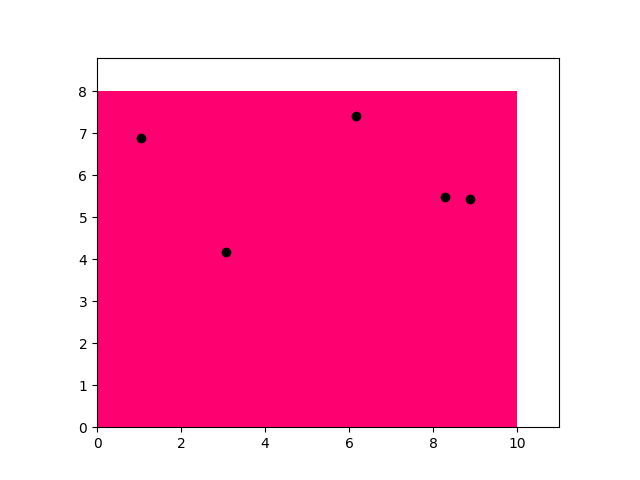
\includegraphics[width=0.8\textwidth]{escena2.png}
    \caption{Cuadro de la animación con cambio de fondo.}
    \label{fig:animacion}
\end{figure}

\section{Análisis e Interpretación}
En la Figura \ref{fig:inicial} se puede ver la distribución inicial de los puntos, la cual es completamente aleatoria. Durante la animación (Figura \ref{fig:animacion}), los puntos se mueven hacia la derecha de forma uniforme. Cuando alguno sale del límite del área, se le asigna una nueva posición dentro del cuadro, lo que permite que el movimiento sea continuo. Además, el cambio de color del fondo se logra de forma sencilla usando un colormap, lo que añade un efecto visual interesante.

\section{Conclusiones}
Esta actividad permitió aprender conceptos básicos sobre el manejo de gráficos y animaciones en Python usando Jupyter y \texttt{matplotlib}. En resumen:
\begin{itemize}
    \item Se logró mover puntos de forma vectorizada.
    \item Se implementó la regeneración de puntos cuando salen del área.
    \item Se añadió un efecto visual al cambiar el color de fondo.
    \item Se consolidó el uso de Jupyter y Python para tareas de simulación.
\end{itemize}



\end{document}
